%
% File acl2019.tex
%
%% Based on the style files for ACL 2018, NAACL 2018/19, which were
%% Based on the style files for ACL-2015, with some improvements
%%  taken from the NAACL-2016 style
%% Based on the style files for ACL-2014, which were, in turn,
%% based on ACL-2013, ACL-2012, ACL-2011, ACL-2010, ACL-IJCNLP-2009,
%% EACL-2009, IJCNLP-2008...
%% Based on the style files for EACL 2006 by
%%e.agirre@ehu.es or Sergi.Balari@uab.es
%% and that of ACL 08 by Joakim Nivre and Noah Smith
% chktex-file 19
% chktex-file 13
% chktex-file 24
% chktex-file 8
% chktex-file 44
% chktex-file 45
% chktex-file 46

\documentclass[11pt,a4paper]{article}
\usepackage[hyperref]{acl2019}
\usepackage{times}
\usepackage{latexsym}
\usepackage{url}

\usepackage{listings}

\lstset{basicstyle=\ttfamily, keywordstyle=\rmfamily\bfseries}

\usepackage[final]{graphicx}
\usepackage{amsmath,amssymb}
\usepackage{algorithm}
\usepackage{pgfplots}
\usepackage{enumerate}
\usepackage{url}
\usepackage[outdir=./]{epstopdf}
\usepackage{flushend}
\usepackage[most]{tcolorbox}
\setlength{\fboxsep}{2pt}
\usepackage[T1]{fontenc}
\usepackage[utf8]{inputenc}
\usepackage[russian,english]{babel}


%\aclfinalcopy % Uncomment this line for the final submission
%\def\aclpaperid{***} %  Enter the acl Paper ID here

%\setlength\titlebox{5cm}
% You can expand the titlebox if you need extra space
% to show all the authors. Please do not make the titlebox
% smaller than 5cm (the original size); we will check this
% in the camera-ready version and ask you to change it back.

\newcommand\BibTeX{B\textsc{ib}\TeX}

\title{Automated Ontology Matching and Construction using Cross-lingual Embeddings}

\author{Denis Gordeev, Alexey Rey, Dmitry Shagarov
	First Author \\
  Affiliation / Address line 1 \\
  Affiliation / Address line 2 \\
  Affiliation / Address line 3 \\
  \texttt{email@domain} \\\And
  Second Author \\
  Affiliation / Address line 1 \\
  Affiliation / Address line 2 \\
  Affiliation / Address line 3 \\
  \texttt{email@domain} \\}

\date{}

\begin{document}
\maketitle
\begin{abstract}
Low-resource languages often lack structured text representations (taxonomies, ontologies and lexical databases) or lag behind in their adoption. In this paper we propose a method for matching and constructing ontologies, taxonomies and other forms of graph-trees with textual information using hierarchical information and cross-lingual embeddings.
\end{abstract}

\section{Introduction}

There are numerous structured information representations containing texts as titles, descriptions or definitions: e.g.\ ontologies, taxonomies, and lexical databases such as WordNet~\cite{wordnet}. Many of them exist only for English, and there have been just as many attempts by researchers to automatically convert such resources from English into other languages. Most attempts were focused on using machine translation engines, bilingual dictionaries or parallel corpora~\cite{Khodak2017,NEALE18.1030}, and results for low-resource languages have been scarce. Some works used word embeddings, which proved a powerful tool for dense text representations after papers by Bengio~\cite{bengio} and Mikolov~\cite{mikolov-representations-2013}. However, first word vector representation models were monolingual only. Soon researchers proposed cross-lingual word embedding models~\cite{mikolov-parallel,lazaridou-parallel}. Unfortunately, most of the early works in this domain relied on massive parallel corpora. This solution is not feasible for low-resource languages due to severe lack of available data.

Learning mappings between embeddings from different languages or sources has proven to be a rather efficient method for solving the data problem to some extent~\cite{ruder-survey}.

Alexis Conneau et al.~\cite{muse} published a programming library called MUSE to map embeddings from two different sources into a single space. They have reached 81.7\% accuracy for English-Spanish and 83.7\% for Spanish-English pairs for top-1500 source queries in a completely unsupervised mode. For English-Russian and Russian-English their results are not as high and they achieved accuracy of 51.7\% and 63.7\% respectively. Their FastText embeddings were trained on Wikipedia datasets for each respective language and do not match the corpora used in ontologies studied in the present paper.

Artetxe, Labaka and Agirre did a study into the limitations of MUSE and showed its results to be low for some language pairs, e.g. English-Finnish (0.38\% accuracy). They also present their own solution called Vecmap~\cite{vecmap} which outperforms MUSE for this task. It gets 37.33\% for Spanish-English on average of 10 runs and 37.60\% as the best result (they estimate MUSE result to be 21.23\% on average of 10 runs and 36.20\% at best) and 32.63\% on average for the English-Finnish language pair.

In this paper we propose a method for matching ontologies, taxonomies and other forms of graph-trees with textual attributes using hierarchical information and cross-lingual embeddings. This approach makes it possible to match ontology graphs containing textual descriptions in different languages. As the example of such a taxonomy pair we use national product classifications: US NIGP-5 and Russian OKPD2. Matching national product classifications is of extreme importance because it lowers transaction costs, facilitates worldwide trade, and helps in bridging the gap between inconsistent product standards in different countries. According to the UN~\cite{unsd} there are at least 909 (the list seems incomplete - e.g.\ the currently used OKPD2 for Russia is not listed) classifications from 159 countries and the bulk of them except the most prominent (and UN-developed) ones are unaligned. OKPD2 is a Russian national classification for goods and services introduced in 2014. It has a four-level hierarchy. Categories consist of a code and its description (e.g. 01.11.11.112 -- Seeds of winter durum wheat where code 01.11.1 corresponds to ``Wheat''). NIGP-5 is its 2-level US analogue (e.g. 620-80 would be ``pens'' and 620 -- ``office supplies'').

Taxonomy/Ontology matching is a rather challenging problem because of the vast number of possible variants of matching which is challenging even for specialists and requires a lot of time. This is also made more difficult by the fact that matching is not one-by-one but many-to-many (some categories from one product classification may be broad enough to correspond to several categories from the other classification) and should be made across several hierarchy levels. Moreover, it requires expert and language knowledge which is especially difficult to come by in cases of rare languages and taxonomies. Thus, our product classification matching algorithm should satisfy several criteria.

Due to the lack of resources for rare languages	the algorithm should be:
\begin{enumerate}

	\item be language independent

	\item not require parallel texts


	Due to the lack of expert knowledge the algorithm should be:

	\item be fully or partially unsupervised
\end{enumerate}

\section{Related work}
There are numerous papers concerned with taxonomies and ontologies matching. There is even a dedicated taxonomy matching competition Ontology Alignment Evaluation Initiative~\cite{ontology-sota}. The winner of the last two years is the model called the AgreementMakerLight~\cite{faria}. It is monolingual only and relies on hash and word matching. Unsupervised WordNet construction has been demonstrated by Khodak in \citeyearpar{Khodak2017}. They use bilingual dictionaries and word embeddings to build Russian WordNet as in our case. The problem of matching product taxonomies was also studied by Gordeev et al.\ in \citeyearpar{gordeev-fruct}.

%\section{Representing graphs as embeddings}
\section{Cross-lingual embeddings}

\begin{figure}

	\centering
	\small
	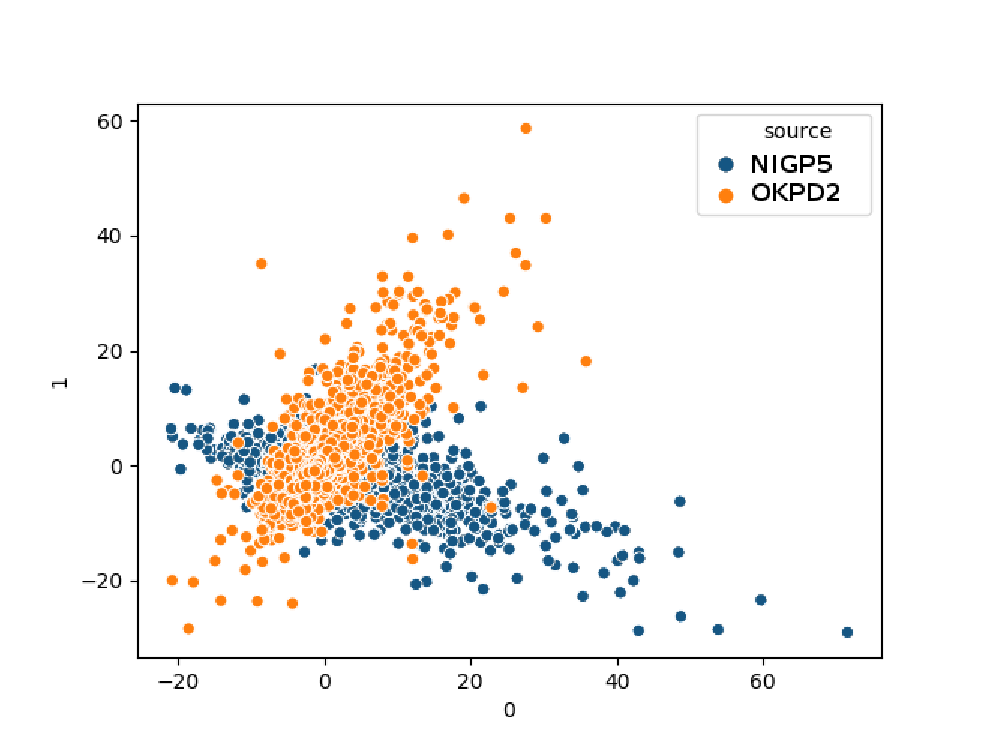
\includegraphics[scale=0.5]{tsne_new}\\

	\caption{PCA visualisation of averaged FastText MUSE vectors for OKPD2 and NIGP-5 taxonomies}
	\label{original-doc2vec}
\end{figure}

MUSE is based on the work by Conneau et al.~\cite{muse}. It consists of two algorithms. The first one which is used only in unsupervised cases is a pair of adversarial neural networks. The first neural network is trained to predict from which distribution $\{X, Y\}$ embeddings come. The second neural networks is trained to modify embeddings $X$ multiplying it by matrix $W$ to prevent the first neural network from making accurate discriminations. Thus, at the end of the training we get a matrix $WX$ which is aligned with matrix $Y$.

The second method is supervised and the aim is to find a linear mapping $W$ between embedding spaces $X$ and $Y$ which can be solved using Orthogonal Procrustes problem:

$$ W^* = argmin_W ||WX - Y||_F = UV^T$$

where $UV^T$ is derived using singular value decomposition SVD$(YX^T) = U \Sigma V^T$
This method is used iteratively with the default number of iterations in MUSE equal to 5. As Søgaard, Ruder and Vulić state Procrustes refinement relies on frequent word pairs to serve as reliable anchors.

Conneau et al.\ also apply cross-domain similarity local scaling to lessen the extent of hubness problem which cross-lingual embeddings are prone to~\cite{dinu}. It uses cosine distance between a source embedding and $k$-target embeddings (the default $k$ in MUSE is 10) instead of the usual cosine distance to generate a dictionary.
$$sim_{source/target} = \dfrac{1}{k}\sum_{i=1}^K\cos(x, nn_i)$$
\small
$$CSLS(x,y) = 2\cos(x,y) - sim_{source}(x)  - sim_{target}(y)$$
\normalsize
Vecmap~\cite{vecmap} is close in its idea to the Procrustes refinement, it computes SVD-factorization SVD$(YX^T) = U\Sigma V^T$ and replaces $X$ and $Y$ with new matrices $X' = U$ and $Y' = V$. The authors also propose normalization and whitening (sphering) transformation. After applying whitening new matrices are equal to:
$X' = {({X^T}X)}^{-\tfrac{1}{2}}$ and $Y' = {({Y^T}Y)}^{-\tfrac{1}{2}}$

Jawanpuria et al.~\cite{jawanpuria} propose a method which is also based on SVD-factorization but in smooth Riemannian manifolds instead of Euclidean space.

Ivan Vulić, Wim De Smet and Marie-Francine Moens  used BiLDA for cross-language information retrieval which is similar to the task of classification matching. In this LDA variant topic distributions are considered to be equivalent for same articles from different languages~\cite{bilda}. However, in our case this method is unlikely to perform adequately because LDA requires longer texts~\cite{short-lda}. Word embeddings methods are preferable for short texts~\cite{maslova-potapov}.

\subsection{Simplistic use of word embeddings for graph representations}
In this paper we use a very simple baseline for representing graphs. We represent higher levels of hierarchy as averaged embeddings of lower levels, thus we use a bottom-up approach. We used cross-lingual embeddings in a single vector space provided by the authors of MUSE (i.e.\ vectors for ``cat'' and its Russian translation \foreignlanguage{russian}{``кот''} are close to each other). Using hierarchical information may be beneficial for a range of text classification tasks~\cite{tax2vec} as well as computer vision problems such as ImageNet~\cite{hedging-bets}. It was also shown by Yang \citeyearpar{glomo} that using knowledge of graphs and hierarchies is beneficial for a lot of downstream tasks such as SQuAD.


%\subsection{Using text information in graph embeddings}
\section{Graph Matching}
There are many methods for graph matching, and quite a few of them are based on graph edit distance. However, they usually make strong assumptions of graph isomorphism. Unfortunately, most taxonomies do not satisfy this assumption (e.g.\ even in cases of a WordNet one word may have different synsets that may be absent from the other language). Inexact matching methods that overcome this constraint are based on spectral decompositions of graphs using eigenvalues or on weighted graph matchings~\cite{30years-graphs}. Given that we deal with cross-lingual embeddings it seemed reasonable to adapt a weight matching algorithm for our task. Thus, we used our hierarchical modification of the so-called Hungarian algorithm~\cite[p.~201]{lawler}~\cite[p.~48]{Riesen2010}. We also compared it with the greedy method, where we just select the vector with the highest similarity.
\subsection{The Hungarian method}
\begin{figure}

	\centering
	\small
	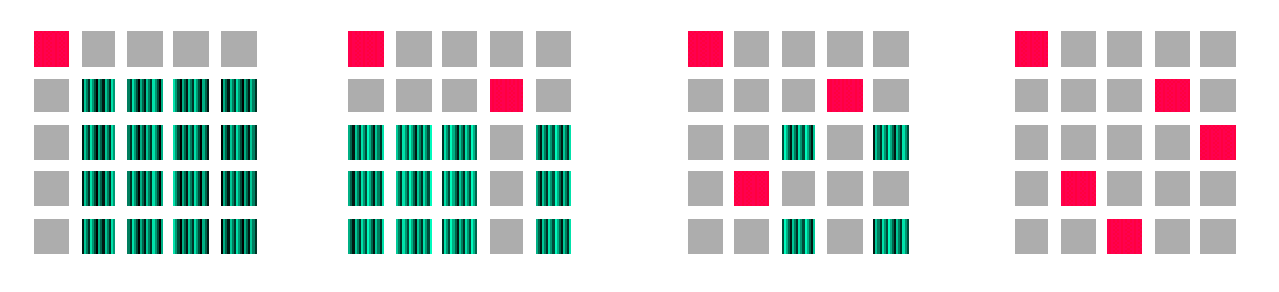
\includegraphics[scale=0.3]{hungarian}\\

	\caption{the Hungarian algorithm visualisation}
	\label{hungarian}
\end{figure}


We use an hierarchical version of the Hungarian algorithm. The algorithm takes as the input a similarity matrix of the size $n \times m$. If $m < n$, the matrix is transposed. As given by Brauner et al.\ in \citeyear{hungarian-listing} the algorithm looks as follows:

1. For the initial weight matrix subtract the minimum from each row and then subtract the minimum from each column.

2. Construct a maximum independent set and a minimal cover of same cardinality k. Exit if k = n.

3. Let $h$ be the minimum of all non covered elements. Add $h=2$ to all elements in each covering line. Then subtract $h=2$ from each noncovered line.This results in $h$ being subtracted from all noncovered elements, and $h$ being added to all doubly covered elements. All entries that are only covered once remain unchanged.

4. Goto step 2.

For each level of the hierarchy we repeat the algorithm. For nodes that were invalidated at the previous (because they correspond to another branch of the tree) similarities are set to 0. If they are still chosen by the algorithm we consider that this node is not present in the graph. Thus, we overcome mismatches between taxonomies/ontologies.
%\begin{lstlisting}[language=Python]
%M: similarity_matrix
%prime_rows = []
%prime_columns = []
%for r in M.rows:
%  min_val = min(r)
%  # delete the min value from
%  # all values of the row
%  r = r - min_val
%for c in M.columns:
%  min_val = min(c)
%  c = c - min_val
%
%\end{lstlisting}

\section{Data}
\subsection{Taxonomies}

\begin{center}
	\begin{table}[!htbp]
		\small
		\caption{Taxonomy examples}
		\label{table-taxonomies}
                \centering
                \begin{tabular}{|p{1cm}|p{2.5cm}|p{2.5cm}|}
                        \hline
                        Category code & Category description \newline (with translation from Russian) & Bid description\\
                        \hline
                        325-25 & Dog and Cat Food & Dog Food: Blue Buffalo Chicken and Brown Rice Food\\
                        \hline
                        43.31.10 & \begin{otherlanguage*}{russian}Работы штукатурные\end{otherlanguage*} \newline Plastering Works & Overhaul of the Basement Of The Administration Building\\
                        \hline
                \end{tabular}
        \end{table}
\end{center}

In this study we use two national product classifications as examples of cross-lingual taxonomies.
Both NIGP-5 and OKPD2 are used to classify products and services. However, they differ in the way products are described (two-level vs four-level hierarchy) as well as in the amount of described categories (8700 for NIGP-5~\cite{wiki-nigp} vs 17416 for OKPD2~\cite{wiki-okpd}). It means that two graphs that might describe these product classifications are not isomorphic (contain the same number of graph vertices connected in the same way and may be transformed into one another).  While it does not imply that they may not be made isomorphic by disregarding some vertices (e.g.\ using some threshold or similarity measure) and then aligned using graph matching methods, it complicates their alignment. It should be also noted that some items from one classification may be completely absent from the other (e.g.\ curd snacks, popular in Russia, or traditional Russian felt footwear `valenki' do not appear in NIGP-5).

The data for the Russian taxonomy OKPD2 was collected from Russian state website Goszakupki\footnote{www.zakupki.gov.ru}, which contains data on procurement awards by government entities.
The data for the US national classification was collected from the US state website data.gov\footnote{https://www.data.gov/}. We have used only marketplace bids by the state of Maryland because they were the only found entries that contained bids descriptions not matching code-descriptions that are required for training Doc2Vec. Extracts from taxonomies can be seen in Table~\ref{table-taxonomies}.

\subsection{WordNet}
We use English WordNet provided by the NLTK package~\cite{wordnet,nltk}. It contains 117'659 synsets. Among them the vast majority does not have hyponyms (97'651) and 30'062 lacks hypernyms (29'716 lacks any hierarchical relations). In this study we examined only nouns (82'115). Because of the small size of the MUSE model we had to use only 22'566 synsets that are included both in the model and in the WordNet.
\section{Experiments}
In this paper we have conducted two experiments. In the first experiment we compared different methods for products taxonomy matching. In the second we used the same methods for unsupervised WordNet construction.
\subsection{NIGP and OKPD2 matching}
Several methods and their combinations were used for mapping taxonomy embeddings. As the first method as described by~\cite{gordeev-fruct}  we tried to train doc2vec embeddings and map them directly using Vecmap or MUSE. However, due to the differences between graphs we failed to reach any meaningful result.

We also made a simple baseline with category descriptions transformed into English using Google Translate. We considered category descriptions from each taxonomy as bags of words, then for a set of words from the first taxonomy we calculated averaged similarity to all category descriptions from the second taxonomy and chose the category from the second taxonomy with the largest similarity. Thus, our method resembles Monge-Elkan similarity~\cite[p.~111]{dupe-detect}:


$$mapping\{A_i, B\}_{i=1}^{|A|} = \max_{j=1}^{|B|}\{sim(A_i,B_j)\}$$

where $$sim = \dfrac{|A_i \cap B_j|}{2} + \\ \dfrac{|B_j \cap A_i|}{2} $$
We used our custom similarity function to fine the function in the cases when the first set of strings is short in comparison with the second set (or the opposite).

We also used hierarchical information to modify mappings from direct string comparison and averaged Word2vec descriptions.

For taxonomy matching using cross-lingual embeddings we tried two approaches: top-down and bottom-up. For the top-down approach we took upper-level category descriptions and transformed them into embeddings using pre-trained MUSE embeddings\ \cite{muse}. We used the averaging scheme (we checked various embedding weighting schemes (e.g. TF-IDF) but did not observe any considerable difference.)
For the bottom-up approach the lowest level of hierarchy was also attained with averaging description embeddings. Upper-level vectors were gained via averaging their constituent node embeddings. As in the top-down approach.
After getting a vector for each category we built layer-wise similarity matrices between taxonomies. Then we applied either Hungarian or greedy method for matching the taxonomies. After getting closest categories for the first layer, we looked only for categories that corresponded to the category chosen at the upper level (e.g.\ if the chosen category code is 64.12 at the next level we look only for categories 64.12.1, 64.12.2).

\subsection{Russian WordNet construction using cross-lingual word embeddings}
We use an extension approach where we take the existing English WordNet and transform its synsets into Russian\ \cite{NEALE18.1030}. As with taxonomies we built a Wordnet tree using hypernym-hyponym relations between synsets. Also we build a list of Russian nouns using the rnnmorph library\footnote{https://github.com/IlyaGusev/rnnmorph}. Then for the bottom WordNet layer we looked for the closest Russian nouns using most-similar function (cosine similarity) provided by the Gensim library~\cite{gensim}. After that, just as in the case with taxonomy matching, we constructed embeddings for the upper level averaging bottom-level vectors. We used the same hyponym-hyperonym relations as for English.
\section{Annotation procedure}

Mappings made by all methods were manually annotated on random 5\% of examples according to the corresponding similarity metric (cosine distance for vectors and our string similarity function for string similarity). The annotation included two classes: True, False. If examples were too specific or too broad (and the annotator was aware of this fact), the match was considered incorrect.
\section{Results}

\subsection{Taxonomy matching}

	\begin{table}[!htbp]
	\small
	\caption{Taxonomy matching results}
	\label{table-taxonomies-results}		
	\centering
	\begin{tabular}{|l|l|l|}
	\hline
	{Method} & {Accuracy \%} \\ \hline
	bottom-up hungarian & 47.5 \\ \hline2
	bottom-up greedy & 45 \\ \hline
	top-down hungarian & 33 \\ \hline
	top-down greedy & 25.5 \\ \hline
	translated strings matching & 41 \\
	\hline
	\end{tabular}

\end{table}

As can be seen from Table~\ref{table-taxonomies-results} the hierarchical Hungarian
method and bottom-up graph embedding representations both help in boosting the results of taxonomy matching. Still translated strings matching is quite a strong baseline which may be the preferred solution when there is a translation engine for the studied language. In the other case the procedure would be: first, to train word-embeddings using some corpora from a common domain (e.g. Wikipedia), then align them using MUSE or Vecmap. After that, those embeddings may be used to map category descriptions. It should be also noted that mappings annotated as wrong were not completely incorrect and were usually on topic (e.g.\ acids -> oils; engine maintenance -> auto body repair; sewage treatment equipment -> sewage treatment services).
We get slightly worse results for string matching in comparison with~\cite{gordeev-fruct} because we use a more rigid annotation procedure and rely on expert knowledge of the taxonomies. Thus, hierarchical information carries more importance in our experiment.
\begin{table*}[ht]
        \small
        \centering
        \caption{WordNet examples}
        \label{table-wordnet-examples}
        \begin{tabular}{|l|l|l|l|}

                \hline
                {Russian child} & {Russian parent} & English child & English parrent \\ \hline
                \foreignlanguage{russian}{экспериментатор} (experimenter)& \foreignlanguage{russian}{физик} (physicist) & \foreignlanguage{russian}{experimenter} & \foreignlanguage{russian}{research worker.n.01} \\ \hline
                \foreignlanguage{russian}{астрофизик} {astrophysicist} & \foreignlanguage{russian}{физик} & \foreignlanguage{russian}{astrophysicist} & \foreignlanguage{russian}{astronomer.n.01} \\ \hline
                \foreignlanguage{russian}{биофизик} (biophysicist)& \foreignlanguage{russian}{физик} & \foreignlanguage{russian}{biophysicist} & \foreignlanguage{russian}{physicist.n.01} \\ \hline

                \foreignlanguage{russian}{рыба} (fish)& \foreignlanguage{russian}{лосось} (salmon) & \foreignlanguage{russian}{panfish} & \foreignlanguage{russian}{fish.n.02} \\ \hline
                \foreignlanguage{russian}{краснопёрка} (redeye)& \foreignlanguage{russian}{лосось} (salmon) & \foreignlanguage{russian}{halibut} & \foreignlanguage{russian}{flatfish.n.01} \\ \hline

                \foreignlanguage{russian}{буксир} (tow)& \foreignlanguage{russian}{катер} (motorboat) & tow & draw.n.09 \\ \hline
                \foreignlanguage{russian}{катамаран} (catamaran)& \foreignlanguage{russian}{катер} (motorboat) & catamaran & sailboat.n.01 \\ \hline

        \end{tabular}
\end{table*}
\begin{center}
       \begin{table*}
		\label{table-annotation}
		\small
		\centering
		\caption{Illustration of category allignment}
		\begin{tabular}{|p{2cm}|p{4cm}|p{2cm}|p{4cm}|p{1cm}|}
			\hline
			{Source Category Code} & {Source Category description}& {Target Category Code} & {Target Category Description (translated from Russian)} & {Result}\\
			\hline
			{800-16} & {Shoes and Boots: Boots, Rubber} &
			{43.31.10} & {\begin{otherlanguage*}{russian}Сапоги резиновые\end{otherlanguage*} \newline Rubber boots} &
			{True}
			\\
			\hline
			958-78 & Management Services Property Management Services &
			{84.11.19.110} & \begin{otherlanguage*}{russian}Услуги государственного управления имуществом\end{otherlanguage*} \newline State property management services &
			Partially True (state)
			\\
			\hline
			936-70 & {Roofing Equipment and Machinery Maintenance and Repair} &
			{33.12.23.000} & \begin{otherlanguage*}{russian}Услуги по ремонту и техническому обслуживанию оборудования для металлургии
			\end{otherlanguage*} \newline Services in repair and maintenance service of the equipment for metallurgy &
			False
			\\
			\hline


		\end{tabular}
	\end{table*}
\end{center}

\begin{table}[ht]
	\small
	\caption{WordNet results}
	\label{table-wordnet-results}
	\begin{tabular}{|l|l|l|}

		\hline
		{Method} & {F1-Score} \\ \hline
		Universal Wordnet & 50.2 \\ \hline
		Extended OpenMultilingual Wordnet & 53 \\ \hline
%a		Khodak & 67.6 \\ \hline
		Cross-lingual embeddings & 66.1 \\
		\hline
	\end{tabular}
\end{table}

\subsection{Wordnet construction}




As can be seen from Table \ref{table-wordnet-results} our results are slightly worse than the ones provided by Khodak. However, our algorithm does not require parallel dictionaries and thus is more applicable to low-resource languages.
Also our method reveals hierarchical relations which are absent from English. For example, it correctly matches `experimenter` and `physicist` because in Russian there is a special synset with this meaning (and they are not always `research workers`). Also sometimes hypernyms and homonyms get messed up and we get that 'salmon' is 'hypernym' for 'fish'.


%14909  экспериментатор     физик    experimenter  research_worker.n.01    0.592080
%15495       астрофизик     физик  astrophysicist       astronomer.n.01    0.783915
%15587         биофизик     физик    biophysicist        physicist.n.01    0.702931
%
%4104          акула    лосось       bowfin          ganoid.n.01    0.586604
%4115        косатка    лосось    snailfish     scorpaenoid.n.01    0.556610
%13042       макрель    лосось        bream  saltwater_fish.n.01    0.637474
%13060          рыба    лосось        squid         seafood.n.01    0.624945
%13066   краснопёрка    лосось      panfish            fish.n.02    0.690515
%13082        тюлень    лосось      halibut        flatfish.n.01    0.617393
%
%184      буксир     катер          tow       draw.n.09    0.571837
%4709  катамаран     катер    catamaran   sailboat.n.01    0.563622


\section{Conclusion}
In this work we have demonstrated several successful methods for unsupervised cross-lingual matching of national product classification systems, we have also shown that the same methods can be used for unsupervised WordNet construction.

The first method taxonomy categories descriptions using a custom string similarity function. Russian category descriptions were converted to English using Google Translate. It performed reasonably well and achieved 41\% accuracy. However, this method is unlikely to be suitable for languages that have less resources and are more distant from English than Russian because of the worse search engine quality for such languages~\cite{google-translate-rare}.


We demonstrate that using translation information from a pre-trained translation engine or using embeddings pre-aligned in a common space may help in solving this task.

We also use a similar method for automatic WordNet construction for the Russian language. We do not get a state-of-the-art result, yet our method does not require bilingual corpora and is, thus, more applicable to a wider range of languages.


\bibliographystyle{acl_natbib}
\bibliography{gordeev}
\end{document}
